\chapter{Design}
\label{design}
The literature has shown us that machine learning methods can be useful in generating feedback for students, and this can be combined with a visual display for intuitive understanding. The first design decision to be made is the language and libraries to be used when writing the program.
\section{Language and Tools}
Two languages are immediate possibilities for implementation: Java\cite{java_site} and Python\cite{python_site}. Java because I had the most experience with it and some parts of Infandango are written in Java. Most of Infandango was, however, written in Python with which I also had experience. Due to the emphasis the project has on machine learning, R\cite{r_site} was another approriate language. 
The final decision was to use Python with scikit-learn\cite{scikit_site} and pybrain\cite{pybrain_site} libraries: this provides the simplest integration with Infandango (since the parts with which this will need to be integrated are written in Python) and the libraries provide a variety of machine learning methods.

\section{Proposed Design}
Using the data from a previous year a model will be trained using machine learning methods. The model will output a value which will be displayed somewhere in the Infandango system. In Chapter \ref{machinelearning} these potential models will be explored further, leading to a decision on which is the best to use in Infandango.
\subsection{Model}
The Infandango system is similar to the Khan Academy system and so the method Khan Academy uses is an approriate starting point. Infandango allows a user to submit many solutions for an exercise, and so does Khan Academy. However, there are two properties that distinguish Khan Academy from Infandango:

\begin{itemize}
\item For each exercise, the next solution submitted is for the same kind of question but the details are randomly generated %MAY NEED TO EXPLAIN THIS
\item A solution is a binary feature: correct or incorrect
\end{itemize}

This means a user can keep submitting solutions to an exercise even after they get one solution correct. However, in Infandango once a user gets 100\% there is no reason for the user to submit another solution because they have already perfected that exercise. The second difference means our data will be numerical instead of binary and this needs to be considered when designing the model.
The first difference is significant, and requires a change in granularity of the data: instead of measuring progress on a submission-by-submission basis, the focus should be on the final mark a user will achieve for an exercise. So instead of trying to predict the score for the next {\it submission}, try to predict the final score for the next {\it question}.

With an idea of how the model was going to work, some exploratory work was done on the data. Although users are encouraged to answer all questions, the do not receive marks directly for each question. This makes missing data a potential problem. Figure \ref{fig:missing_data} shows the submission rates for all the questions. It shows that submission rates can get as low as around 10\% for some questions. Figure \ref{fig:missing_data_core} shows the submission rates for only core questions. The submission rates are on average higher than for non-core questions. Combined with the fact that users are likely to have more motivation for core questions (since they potentially count towards their final mark) data from now on will only be considering core questions.

\begin{figure}[b!] 
\centering
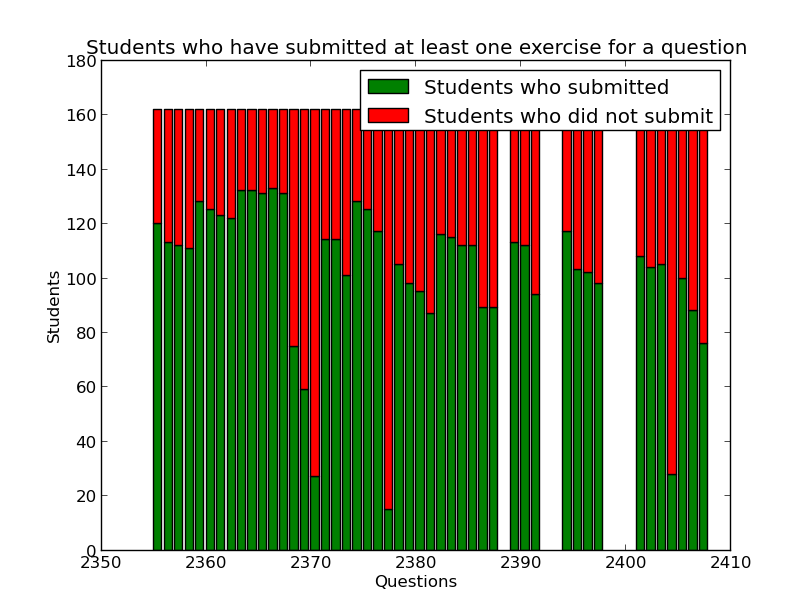
\includegraphics[width=0.8\textwidth]{images/missing_data.png}
\caption{Submission rates for all questions}
\label{fig:missing_data}
\end{figure}

\begin{figure}[b!]
\centering
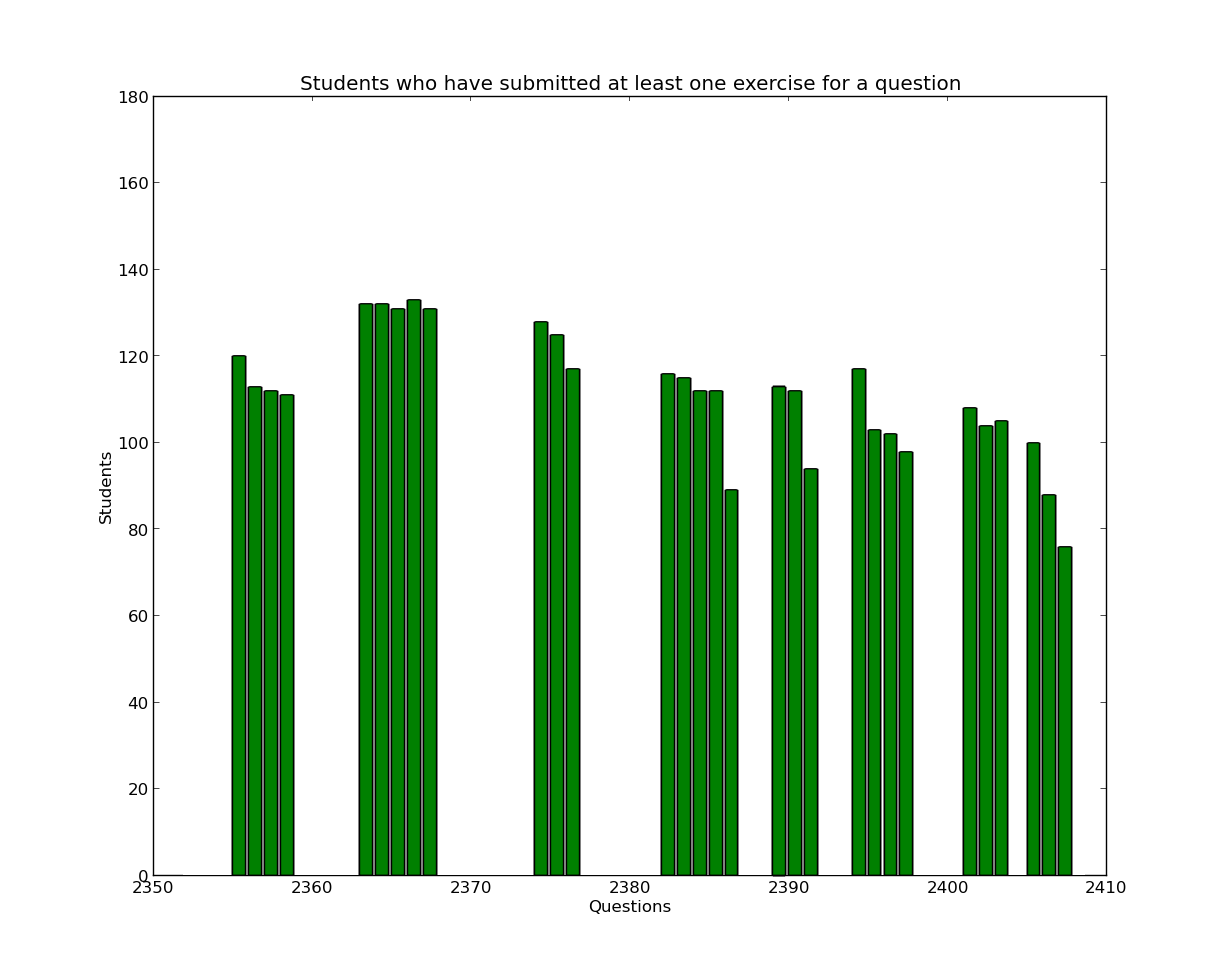
\includegraphics[width=0.8\textwidth]{images/missing_data_core.png}
\caption{Submission rates for only core questions}
\label{fig:missing_data_core}
\end{figure}

\begin{figure}[b!]
\centering
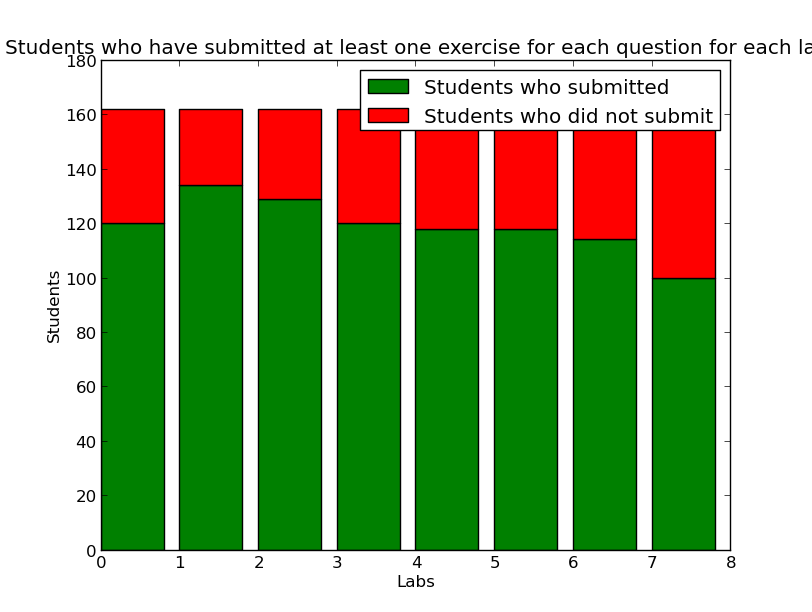
\includegraphics[width=0.8\textwidth]{images/missing_data_week_any.png}
\caption{Submission rates for at least one question per week}
\label{fig:missing_data_week_any}
\end{figure}

With the amount of missing data still being significant changing to yet another level of granularity was considered: predicting on a week-by-week basis. Using this method there could be a lot less missing data: take the average of all the questions for a week to get the score for that week. This means there will still be a data point for a student if they miss one question, and they would have to have no solutions for all questions in a week to get no score for a week. Comparing Figure \ref{fig:missing_data_week_any} to Figure \ref{fig:missing_data_core} a rise in the amount of data points can be seen. On average there is about 115 data points for a given week, and about 100 data points for a given question.

Although this does provide slightly higher yield there are disadvantages to predicting on a week-by-week basis:

\begin{enumerate}
\item It would take a week before there was even one data point to start giving feedback from
\item Feedback would only be updated weekly. After a student has been working on questions for a few days the feedback is likely to be outdated
\item A separate model would need to be trained for each week. To predict the score for week 3 you want to use two features: the score for weeks 1 and 2. For week 8 you would like to use all the available features: weeks 1 to 7. Having a variable number of features means having different models for each week
\end{enumerate}

Problems 1 and 2 are not really present if prediction is done question-by-question. Problem 3, however is still present: a new model needs to be trained for each question. A solution to this problem will be discussed later.

\subsubsection{Identity based features}
Starting with the Khan Academy model and adapting it based on Infandango and the available data a model can be proposed for Infandango: For each question, train a new model which takes all previous questions as input features. The model then tries to predict the score for that question.

\subsubsection{Moving Window}
Previously an assumption has been made: the identity of the question is necessary. While the identity of the question is likely to be important it is not necessary and removing this constraint allows a simple, singular alternative model to be proposed: The model always has N features and tries to predict the score of the N+1 question. For the simplicity of the following description N = 5 will be assumed.
There are 5 input features. The features will be decided based on their locality to the output feature: if we want to make a prediction for question 6 then the input features will be questions 1, 2, 3, 4 and 5. All the input features occur before question 6 because when a student is completing questions they are much more likely to do them in order, and so questions 7, 8 and 9 are not likely to present when making predictions. 
Although this approach does remove the significant information of the identity of the questions it is simple to implement and it also provides a lot more training data: There are 30 questions, and so using this approach for each student there would be 25 potential training examples. However, using the previous model there would only be 1 item for each model.



\subsection{Visualisation}

\section{Integration with Infandango}
The final step in completing the project is to integrate the system with Infandango. This is a non-trivial task whose outcome will determine the future usability of this addition to the system. Infandango uses Django to generate the information which is displayed via HTML and CSS. This includes information such as the submissions and the scores received for each submission. The feedback score is of a similar nature so, in line with the design of Infandango, the feedback score will be displayed using HTML and CSS after being generated via Django. The precise details of this integration will be discussion in Chapter \ref{implementation}.
